\begin{comment}
\section{Quality-Centric Data Model}
\todo{Rewrite Introduction}
In this section I will start presenting the \textit{quality-centric data model} we have developed, with
the aim of increasing the system \textit{dependability} and to reason about the achieved
\textit{quality-of-service}.
I will first describe a novel metric called \textit{Source \DIFdelbegin \DIFdel{Information Content}\DIFdelend \DIFaddbegin \DIFadd{Coverage Ratio}\DIFaddend } (\sic), which is a
metadata value associated with data streams. Then I will provide some foundation assumptions we made in
the design of it and the reasoning behind these decisions.
\end{comment}

\begin{comment}
\DIFdelbegin %DIFDELCMD < \subsection***{Source Information Content}
%DIFDELCMD < %%%
\DIFdelend \DIFaddbegin \subsection***{Source Coverage Ratio}
\DIFaddend 

In a traditional stream processing system streams only contain data associated with
timestamps, they do not carry information about the failure experienced by the system. In our model we
propose to augment streams so that failure is recorded and accounted for. In order to do so we introduce
a new metric called \textit{Source \DIFdelbegin \DIFdel{Information Content}\DIFdelend \DIFaddbegin \DIFadd{Coverage Ratio}\DIFaddend } (\sic) that gives a hint about the amount of
information contained in a tuple and thus to its importance for the current query results. This is added
to streams in the form metadata, whose value is calculated by the query operators and is inversly
proportional to the occurrence of failure.

A tuple should convey information about the amount of failure experienced during its creation. There
should be a way to indicate if the data carried by a tuple was created using all the available
information, and is then 100\% accurate, or if some information was lost in the process, thus reducing
the dependability of that data. \textit{Source \DIFdelbegin \DIFdel{Information Content}\DIFdelend \DIFaddbegin \DIFadd{Coverage Ratio}\DIFaddend } tries to do achieve
this goal, by measuring the amount of lost information in the creation of a tuple.

The system can use this value to make decision about the importance of a tuple towards the creation of
the final query result. When the system is overloaded for instance, it has to decide which tuples should
be dropped in order to recover. \sic values in this case can be used to assess the individual value of
tuples and guide the system to a selection that helps improving the quality of the results.

In a single query scenario the system is able to reason about the amount of information carried by
tuples, by dropping the ones with the lowest values it minimises the impact on the query results. Even in
the absence of failure it may be that some tuples aggregate more information than others and should be
treated with more care. In case of failure then, the system would prefer to drop some already compromised
tuples before other which where produced with perfect information.

When dealing with a system that allows the the concurrent execution of multiple queries, \sic values
help discarding tuples so that all queries in the system are affected in the same way. All qu
This process is referred to as  \textit{fair shedding} and will be further analysed in
Section~\ref{sec:fair shedding}.

In the next section I will present some assumption we made about the \sic quality metric, giving some
reasoning behind them. I will not introduce any formulas at this point, leaving the discussion about how
\sic values are c alculated to Section~\ref{sec:sic}.
\\
\end{comment}

\section{Model Assumptions}
\label{sec:assumptions}

% In the design of a suitable quality metric that could be used to capture the amount of failure
% occurring in the processing of a query, there need to be some assumptions that limit and define it.
This section states the assumptions that led to the definition of a quality metric called Source
Information Content (\sic), which is presented formally in Section~\ref{sec:sic}.
It is based on the consideration that overload is a common condition and should not be ignored but
accounted for. Instead of trying to mask it, the system should monitor it and report its impact.
Since queries can be composed of an arbitrary set of operators, frequently employing diverse processing
semantics, a quality metric must be sufficiently generic to be usable across the whole spectrum of
possible queries and not tied to a specific domain. \\
When considering data sources, it is possible that some of the produced inputs are more valuable than
others but it is often difficult to decide this beforehand. The challenge of determining which sources
and tuples are more valuable than others leads to the idea of considering all tuples as equally
important. When an operator receives some tuples as input, it transforms them but does not change the
amount of information that they carry.
Conceptually, this is similar to the conservation of energy law in physics.
Another consideration is that the amount of information in a tuple is proportional to the amount of
tuples required for its generation. Since we assume that every source produces the same amount of
information per time interval, the total amount of information processed by a query in the absence of
failure is a multiple of the number of sources. Finally, we consider the shape of a query graph, which,
in its most generic form, is a directed acyclic graph. The computation of the quality metric should be
flexible enough to be usable for all graphs. \\
The rest of the section describes these assumptions in more detail, laying out the reasoning that lead to
the Source \DIFdelbegin \DIFdel{Information Content }\DIFdelend \DIFaddbegin \DIFadd{Coverage Ratio }\DIFaddend (\sic) quality metric.\\

\textbf{1. FAILURE IS EVERYWHERE\\ \textit{Failure is always present in large-scale query processing,
and overload is a kind of failure.}}

  In large-scale distributed systems, failure cannot be considered a rare and transient condition.
  In fact, evidence suggests that, in such systems, a certain percentage of nodes will be failing at
  all times. Even though the Mean Time Between Failure (MTBF) for a single component may be quite high,
  once the number of components increases, failures become more and more relevant. 

  In a paper released by Google~\cite{google-failure-disks}, it is shown how the occurrence of failure in
  a large hard disk population is higher than what is declared by vendors. They analyse a large
  population of disks and showed how the Annualized Failure Rate (AFR) ranges from 1.7\% for first-year
  drives to over 8.6\% for three-year old drives.
  Jeff Dean of Google also presents statistics~\cite{google-failure-talk} about the real world occurrence
  of failure in their data centres, showing that a typical cluster of 2400 machines it is expected to
  experience around 1000 individual machines failures in the first year alone. 
%   There is a 50\% chance that a cluster overheats, taking down most of the servers in less than 5 minutes
%   and taking 1 to 2 days to recover.
%   
  Overload can be considered as a type of failure because the system cannot process all the
  incoming data and must discard some of it. In this case, an approximate result is produced even
  though all the processing units function correctly.
  Input data rates can be highly unpredictable, with variations that can often be of orders of
  magnitude~\cite{load-shedding}. This makes it challenging to provision a system. 
  If we consider a cloud deployment scenario, in which resources are rented, overload can not
  only be tolerated but may be deliberate. It may be cheaper to underprovision the system on purpose in
  order to keep the costs down when the approximation of results is not an issue.  
  In case of a federated resource pool, in which several parties share their local clusters to gain access
  to a unified processing infrastructure, the possibilities for overload are even higher. Each local
  site, in fact, is under the control of a different authority, making recovery
  times unpredictable. Due to its nature as a shared platform, the processing resources available at each
  cluster are not uniform. The query fragments distributed across several processing sites thus
  experience a skewed availability of resources. For example, the same query fragment may run without failure at one
  site, while experiencing heavy overload at another.\\

\textbf{2. APPROXIMATE PROCESSING \\ \textit{Users can accept approximate processing but they need to have a
way of evaluating the quality of the computed results.}}

 	Failure should be considered a normal condition of operation for a large data stream processing
	system. We propose to augment data streams with a metric that captures the amount of failure during
	the processing. This quantifies the impact of failure instead of hiding it. 
	In many applications, an approximate result is acceptable for users. It is up to the user to decide if the quality
	of the delivered results is good enough for these to be accepted or if they should be discarded.

In sensor networks, it is common to have a lot of failure at the data source level. Sensors can suddenly
stop working because of hardware failure or can become temporarily unreachable. In such cases, a query
that processes sensor readings delivers results that are incomplete. Nevertheless, the quality of the
query results can be sufficient to be meaningful to the user. Especially when dealing with a large set of
sensors, the lack of input from a certain number of them does not mean that the computation should be
discarded altogether. Instead, the results become less accurate due to the missing input data. If we
consider queries aggregating readings for sensors scattered over a geographic area, such as an average of
measured pollutants in a city, it is possible that a failed sensor is located close to others that
record an equivalent reading. Thus the missing information may not produce a significant variation in the final
result, which is approximate yet still meaningful.

If we consider queries that detect a certain event instead, the failure of a single sensor can become
critical. The failed sensor could be the one that would have generated a reading of interest but, due to
the failure, this reading is not available. In this scenario, failure reduces a user's confidence in the
results and may not be tolerable. Even if an approximation of the results may not be acceptable, it is
important to notify the user that some failure occurred during the collection of the input data, leaving
the final decision about the confidence in the results to the user.

An analogous argument can be made for the social media analysis scenario. In this case, the enormous
amount of available input data can cause an overload condition of the processing infrastructure.
Unlike the sensor data scenario, in which the failure usually occurs at the input level, the failure here
is more likely to happen at the processing stage. Aggregation queries typically process vast amounts of
data and, in case of the loss of a small percentage of data, they can still produce results close to what
would have been obtained in the absence of failure. In general, when dealing with aggregation, the larger
the set of input data, the more tolerable failure becomes.\\

\textbf{3. A GENERIC QUALITY METRIC \\ \DIFdelbegin \textit{\DIFdel{A quality metric should be operator independent, abstracting from
the query semantics.}}%DIFAUXCMD
\DIFdelend \DIFaddbegin \textit{\DIFadd{A quality metric should be operator independent, abstracting
the query semantics.}}\DIFaddend }

Stream processing systems are versatile and can compute a variety of queries. Each query is composed of
operators whose semantics can be different. If we consider the streaming equivalent of traditional
operators present in a relational DBMS, such as \textit{filter} and \textit{average}, it is notable how
the discarding of a tuple from the input of these operators can lead to significantly different quality
reductions in the produced output. Due to their different processing semantics, missing a single tuple
can have almost no influence or can completely alter the output of an operator.
Furthermore, it is common for stream processing systems to be extensible, allowing users to implement
their own custom operators, whose processing semantics are unknown a priori.

Let us consider the different impact that the loss of a tuple can have on operator results.
An average operator \DIFdelbegin \DIFdel{, }\DIFdelend that inputs a set of $100$ tuples with integer values uniformly distributed in the
range $[0,1]$, produces a single output tuple with a value close to $0.5$.
If we assume that $50\%$ of the input tuples are discarded due to overload, the operator still produces a
single tuple with a value close to $0.5$. In this scenario, the loss of half of the input tuples has
virtually no impact.

A filter operator with the same input tuples outputs only tuples with values below $0.5$. Since
the input is uniformly distributed, it produces on average an output of $50$ tuples.
When shedding half of the input values though, the operator result changes considerably. On average, it
now produces $25$ output tuples, which is half of the number of tuples that it would produce with the
complete set of input tuples. With this simple example, we can observe how the processing semantics of
the operator can be different: the impact of input loss can be almost unnoticeable for some operators
while it can be disruptive for others.

Therefore, the quality metric should be operator independent and valid for any kind of processing
semantics, efficiently capturing the processing degradation under failure. Even though the knowledge of
the internal functioning of operators would allow the system to have a more precise reasoning about the
impact of failure on the quality of the results, this is impractical for a general purpose system.
Instead of trying to quantify the approximation of the result in terms of  precision, we try to quantify
the amount of information that was lost during the computation of a result compared to the total amount
that would have been processed in the absence of failure.

Other \DIFdelbegin \DIFdel{proposal }\DIFdelend \DIFaddbegin \DIFadd{proposals }\DIFaddend for an operator independent approach exists. The \textit{network imprecision}  metric
accounts for the state of all participating nodes in a large-scale monitoring
system~\cite{network-imprecision}.
It estimates the percentage of nodes available when calculating an aggregate value over a set of data
sources. In contrast, our metric operates at the granularity of individual tuples, not sources, to reason
about the impact of information loss on the results.
Another example is the \textit{harvest} quality metric proposed by Murty and
Welsh~\cite{dependable-is-sensing} and Fox and Brewer~\cite{Fox1999}. The authors argue that harvest
should capture the fraction of data sources available in an Internet-scale sensor system. \\

\textbf{4. DATA SOURCE EQUALITY \\ \textit{All sources are equally important for the generation of the
final result data.}}

In our model, sources are all considered equally important, regardless of their tuple production rate.
If we consider a sensor network deployment, it is common to observe different rates of input readings.
This is due to different sensor settings or different battery constraints of the sensors. A unit with a
depleted battery may reduce the rate at which it propagates information to save energy.
Another reason could be the position of a sensor. The energy cost of propagating a reading grows with
distance because it requires a higher transmission power.

	Consider a sensor network monitoring humidity levels in a rural area, composed of sensors randomly
	scattered over a certain region. The processing query produces an average humidity value for the area
	every hour, aggregating readings from all sensors, which are produced once every $10$
	minutes. Due to the uneven distribution of sensors, some may require more power to transmit their
	readings and, in order to save battery power, may decide to reduce their transmission rate to half the original rate. 
	When aggregating the humidity values, the amount of tuples for each sensor would be different. The
	processing query would first group the readings by sensor id, average a single result for each sensor
	over the specified time window, and finally compute a global average. We can see this as an average
	over a single reading from every sensor, each conveying information about a certain location but with
	a different resolution. Nevertheless, the information produced by all sensors has the same value for the
	final calculation of the global humidity value.

	In the previous example, all tuples generated by a sensor in a one hour time-window convey the same
	information, regardless of the fact that some sources produce more tuples than others. All
	sources equally contribute to the final result.

	In our model, we treat all sources as equal but this is not valid in all cases. There may
	be scenarios in which a particular source should be considered more important than others. For
	example, it may be placed in a strategic location or it may be equipped with a more
	sophisticated sensor. \\
% 	A possible extension to our model that would account for this
% 	differences is to include a \textit{weight} parameter. This would allow the user to indicate to the
% 	system which tuples should be regarded are more valuable. The system then would assign a different
% 	importance to these tuples and try to avoid dropping them, with a probability proportional to their
% 	weight. 

\textbf{5. TUPLE EQUALITY \\ \textit{All tuples from a data source are equally important for the generation
of the final result.}}

	All tuples produced by a data source that lead to the creation of the same result are considered to contain
	the same amount of information. Since our model abstracts from the semantics of the query and is
	designed to be used for generic queries, it treats all source tuples as equal. 
	%This means that in case of overload it would make a random decision about which tuples to drop.

Let us consider a simple query, composed of one data source and one average operator, producing a single
result every minute. The source produces $1000$ tuples per second. The system is overloaded and unable
to process all of the tuples. If the distribution of values carried by the source tuples is uniform, it
does not make a difference which tuples are discarded. If instead the distribution is highly skewed,
including a small number of outliers, discarding one of them could significantly change the aggregated
result. Since the system employs an operator independent model, it cannot know which tuples to drop in
order to reduce the error of the results. 
%Therefore, it treats all source tuples as equal and makes a random decision.

This is a simplification to keep the model abstract enough to be usable in a general purpose system. Of
course, there are situations, such as when using detection queries, in which some source tuples are more
important than others. Having the knowledge of the query semantics could enable the system to be more
selective and make distinctions between tuples when making shedding decisions but it would limit the
system to support a set of operators and queries.

A tuple acquires more value when it is obtained through the processing of many other tuples. The tuple
equality principle only applies to source tuples and not derived tuples. Derived tuples are obtained as
output from operators and their value is proportional to the amount of information (\ie the number of source
tuples) that they aggregate. In Chapter~\ref{ch:load_shedding}, the difference in terms of information content among derived tuples is exploited
to implement an intelligent overload management strategy. \\

\textbf{6. CONSERVATION OF INFORMATION \\ \textit{The amount of information going into an operator is
equal to the amount of its output, regardless of the number of tuples produced.}}

An operator processes one or more input batches and produces a single output batch. Every tuple that
enters an operator has a certain value for its quality metadata.  It is the same for all tuples in a
batch and may be different for different batches. The operator transforms these tuples into a new set
according to its processing semantics. Even though the amount of tuples in the output may be different from
the amount in its input, the \textit{amount of information} does not change. We assume that the
total value for the quality metric in the input to an operator is not changed by the processing and is
transmitted to the output tuples.

 	Let us consider a simple \textit{map} operator, which transforms a Fahrenheit temperature reading into
 	its Celsius equivalent. This operator receives $N$ tuples as input, applies a simple equation and
 	produces $N$ tuples as output. The information carried by the input tuples is transformed but its
 	total amount does not change. 

Another class of operators deals with \textit{aggregation}. We can use a simple average as representative
example. Such an operator receives $N$ tuples as input and produces a single output tuple.
Consider an operator calculating the average temperature in a room every minute. It receives all the
input tuples produced by the sensors during the specified time window and outputs a single average value.
Even though only a single output tuple is produced, it carries all the information for the input tuples,
transformed into only a single aggregate value.

Consider a \textit{filter} operator, which discards a certain number of tuples that do not satisfy a set
of predicates. As an example, we can imagine an operator filtering all temperature readings with a value
below $30$ degrees Celsius. As input, it receives $10$ tuples, out of which only $5$ carry a reading
above $30$ degrees. The number of output tuples in this case is only 50\% of the input, yet the total
information carried remains unchanged. What changes is the individual information value associated with
the single tuples, which is doubled compared to when the tuples entered the operator.

In all the previous examples, the number of tuples produces by an operator was smaller or equal to the
number in the input. This is not true for all operators though. If we consider a \textit{join} operator,
the number of tuples in the output can be greater than in the input. Let us consider a join
operator that has one input with temperature readings for a given room and another with
humidity values. The tuples from the first input have a schema $\langle\textsc{RoomID, Tmp} \rangle$,
while the second input has a schema $\langle\textsc{RoomID, Humidity}\rangle$. The operator joins the two
streams on the field \textsc{RoomID}, producing a stream of output tuples with schema
$\langle\textsc{RoomID, Tmp, Humidity}\rangle$. The amount of tuples produced by this operator is in the
range $[0, N{\times} M]$, where $N$ is the number of temperature tuples and $M$ the number of humidity
tuples.
This means that it is possible for such an operator to produce more tuples in its output than in its
input. From the perspective of our model, the information is still preserved, even though the individual
quality values of tuples decreased.

 	Finally, we consider the case, in which an operator produces no output at all. This can happen
 	with filtering operators, when all the input tuples do not satisfy the filtering predicate and therefore
 	are discarded. Since there is no output tuple to carry the input information content, this case
 	would be indistinguishable from the case where all the input tuples have been lost, for example, because the
 	system decided to discard them to overcome an overload condition. In this case, the system
 	still needs to produce an \textit{empty batch}, containing no tuples but with a total quality metadata
 	value equal to the sum of the values received in the input. In this way, the total amount of
 	information is preserved. \\

\textbf{7. INFORMATION IS VALUE \\ \textit{The importance of a tuple is directly proportional to the
amount of information required to generate it.}}

\begin{figure}[b!]
	\centering
	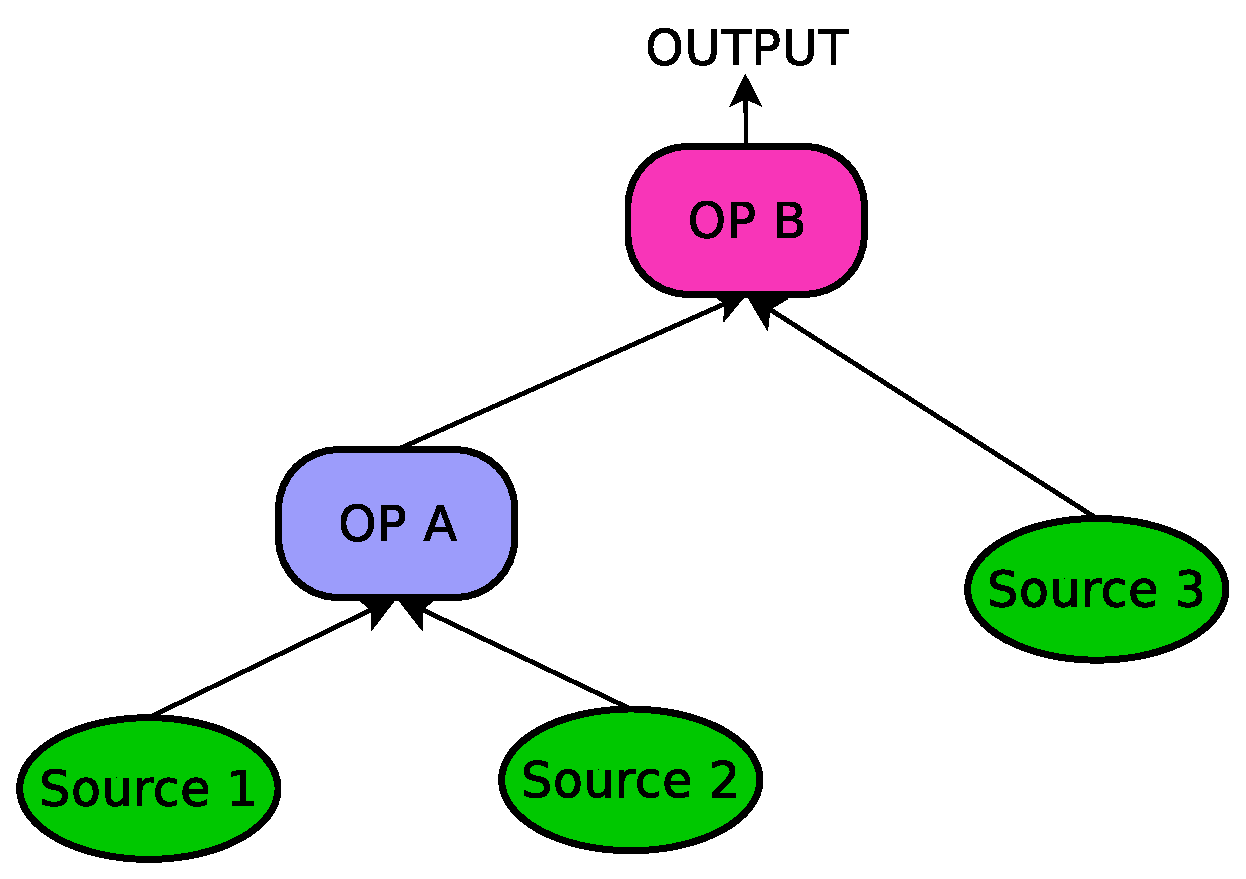
\includegraphics[width=0.55\textwidth]{img/tesi/unbalanced-tree_senza}
	\caption{An unbalanced query tree, showing the different information content of tuples.}
	\label{fig:unbalanced-tree}
\end{figure}

	
	When we consider the importance of an individual tuple within a query, it is important to take into account the
	amount of information that went into its creation. The more information is part of a tuple, the 
	more important it becomes for the computation of the final query result. If the system needs to make a
	decision about which tuples to discard, it has to consider the individual information content of tuples and
	discard the ones with the lowest values first. This is done to reduce the amount of missing information in
	the final query result. 

Let us consider a query whose graph representation resembles an unbalanced tree, as shown in
\mbox{Figure~\ref{fig:unbalanced-tree}}. In this query there are $3$ sources, all producing tuples at the
same rate. The input tuples produced by source 1 and 2 are first combined together by operator A. The
resulting tuples are processed by operator B, together with the tuple produces by source number $3$.
We can assume that the operator B resides on a different machine than operator A and that, due to
overload, it needs to discard one tuple out of the four present in its input buffers. When comparing the
information values of the tuples, the tuples received for the left input stream have an information
content that is twice that of the tuples received on its right input stream. This is because the tuples
on the left contain the information for $2$ sources, while the others carry the
information for a single source. Since the goal of the system is to deliver results with the maximum
amount of source information, the system decides that the tuple to discard should be one of those
received on its right input. \\

\textbf{8. TOTAL INFORMATION CONTENT \\ \textit{The total amount of information contained in a result in
the absence of failure is equal to the number of sources}}

In the absence of failure, every result batch produced by a query contains an amount of information that
is equal to the sum of the individual information values carried by the source tuples.
Considering every source as equal, we can assign a value of $1$ to the complete set of source tuples for
each source that contributed to the calculation of a result batch. If we do so, the final value of a
result batch is equal to the number of sources.

	Let us consider a simple query that calculates an average pollution value every minute from a set of
	$10$ sensors located at different locations in a city. This query produces a result batch of a single tuple,
	which aggregates all the information gathered by the $10$~sensors over a one minute window. Let us
	assume that no failure has happened and that all tuples are correctly processed. Since all sources are
	considered equal, the total amount of information carried by the tuples produced by each source
	over a minute is $1$. When the final result is computed, the total information is equal
	to $10$ (\ie the number of sources).

	When dealing with a system that supports the concurrent execution of multiple queries, it becomes
	important to compare the information values of the different queries. This is needed in
	an overload condition, when trying to achieve \textit{fair shedding}. In fair shedding, the system
	selectively discards tuples to reduce the load of the system so that the final quality values of all
	queries is equalised.
	Therefore, the system must compare the different information content values of tuples. A simple
	way to achieve this is to normalise the information content value by dividing the total
	value of a query result by its number of sources.
	This scales all values in the interval $[0,1]$, making them comparable.\\

\textbf{9. QUERIES ARE DIRECTED ACYCLIC GRAPHS \\ \textit{An operator may have more than one downstream
operator.}}

	A query can be represented as a directed acyclic graph (DAG), in which nodes represent operators and
	arrows the streams flowing through them. This means that, as long as there are no cycles, every operator
	can have multiple downstream operators that receive its output as input. There are two reasons for
	distributing the output of an operator: (1) the query has to compute multiple results; and (2) the
	downstream computation has to be split over multiple machines because it would be too computationally
	intensive for a single one.

The first case deals with queries computing multiple results. These are called \textit{fan-out} queries
and will be further discussed in Section~\ref{sec:fan-out}. They compute multiple results based on common
input information but are logically a single query. The reason for treating a query with multiple results
as a single query is to allow the system to be fair when making shedding decisions under overload.
Let us consider a system with two running queries, submitted by two users. The first user submits a
query with a single terminal operator, while the query submitted by the other user may have $9$.
If the system considered each computed result as a single query, the second user would be allocated 90\%
of the available resources, leaving only 10\% to the first. If the system instead considers the query
submitted by the second user as single computation with $9$ different results, it can evenly discard
tuples among the two queries, leading to a fair allocation of the available computing resources.
Fair shedding will be described in more detail in Section~\ref{sec:fair-shedding}.

	The second reason for the distribution of the output of an operator is when the downstream computation
	is too intensive to be executed by a single machine. In this case, the output is split among several
	processing nodes, each hosting the same set of operators that process a fraction of the output
	tuples.
	The computed results are then collected to produce a single final result. 

	When computing the values of the quality metric, the system needs to take this into account. In
	particular, an operator distributes the total value of information from its input to all its output
	tuples.
	A tuple is assigned a value that is inversely proportional to the number of the output streams of the
	operator. In the first case, when multiple results are calculated, each terminal operator will produce
	tuples with a value equal to the number of sources, divided by the number of results. In this way, the
	cumulative information value for the query is the same as in cases with only a single terminal
	operator.
	The details of this are covered in Section~\ref{sec:sic}.
